\subsubsection{Aktivitet og intensitet}
Der findes en klar sammenhæng imellem puls og kroppens reaktion på motionen. Ifølge flere studier hænger procenten af den maksimale puls sammen med, antallet af forbrændte kalorier, om den aerobe udholdenhed trænes, forbedrer den anaerobe tolerance eller forbedrer den cardiovaskulære ydeevne\fxnote{hvilket gør, at man kan sprinte længere / er hurtigere, fordi der kommer mere ilt rundt i kroppen}. Jo højere procent intensitet, desto højere puls og hårdere fysisk træning. Denne sammenhæng inddeles i zoner som ses på \tabref{tab:PA_Procentpuls}. \citep{Leyland2007,Heartratejournal2015}
%\begin{figure}[H]
%	\centering
%	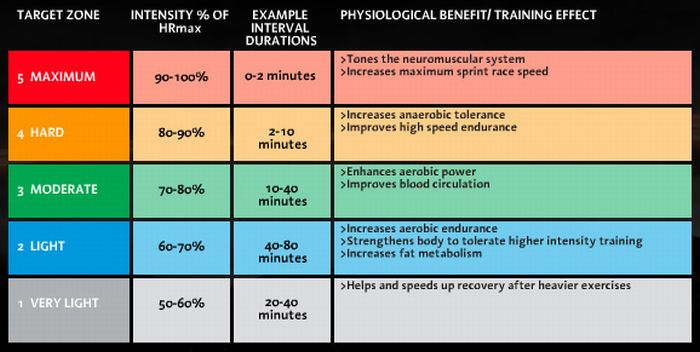
\includegraphics[scale=0.75]{figures/aProblemanalyse/heart-rate-zones.jpg}
%	\caption{På figuren ses fem zoner for kroppens reaktion i forhold til pulsraten. Der ses, at de fem zoner har hver sin påvirkning på kroppen. Det er dog også anbefalet, at varigheden i hver zone bliver lavere desto hårdere aktiviteten er. \citep{Heartratejournal2015}}
%	\label{fig:PA_Procentpuls}
%\end{figure}
\begin{table}[H]
	\centering
	\resizebox{\textwidth}{!}{%
	\begin{tabular}{@{}lll@{}}
		\rowcolor[HTML]{C0C0C0} 
		\multicolumn{1}{c}{\cellcolor[HTML]{C0C0C0}Zoner} & \multicolumn{1}{c}{\cellcolor[HTML]{C0C0C0}\begin{tabular}[c]{@{}c@{}}Intensitet \%\\ af maxpuls\end{tabular}} & \multicolumn{1}{c}{\cellcolor[HTML]{C0C0C0}Fysisk effekter}    \\
		\multicolumn{1}{l}{5 - Maksimum}                & \multicolumn{1}{l}{90-100 \%}           & \multicolumn{1}{l}{Træner det neuromuskulære system og øger maksimal sprinthastighed.}   \\ \hline
		\multicolumn{1}{l}{4 - Hård}                    & \multicolumn{1}{l}{80-90 \%}  & \multicolumn{1}{l}{Forbedrer den anaerobe tolerance og øger højhastigheds udholdenhed.}     \\ \hline
		\multicolumn{1}{l}{3 - Moderat}                 & \multicolumn{1}{l}{70-80 \%}  & \multicolumn{1}{l}{Øger aerob power og forbedrer blodcirkulationen.}      \\ \hline
		\multicolumn{1}{l}{2 - Let}                     & \multicolumn{1}{l}{60-70 \%}  & \multicolumn{1}{l}{\begin{tabular}[c]{@{}l@{}}Forbedrer den aerobe udholdenhed, styrker kroppen til høj intens\\ arbejde og øger fedtmetabolismen.\end{tabular}} \\ \hline
		\multicolumn{1}{l}{1 - Meget let}               & \multicolumn{1}{l}{50-60 \%}  & \multicolumn{1}{l}{Hjælper og øger hastigheden af genopbygningen af musklerne efter hårdt træning.}   \\ \hline
	\end{tabular}
	}
	\caption{I tabellen ses fem zoner for kroppens reaktion i forhold til pulsraten. Der ses, at de fem zoner har hver sin påvirkning på kroppen. Det er dog også anbefalet, at varigheden i hver zone bliver lavere desto hårdere aktiviteten er.\textit{(Revideret)} \citep{Heartratejournal2015}}
	\label{tab:PA_Procentpuls}
\end{table}

Det er dog omdiskuteret, hvorvidt zone 1 og 2 er de fortrukne, hvis ønsket er at tabe sig. Der forbrændes flere kalorier ved højintens aktivitet, altså i zone 4-5. I de lavintense zoner forbrændes kalorier fra fedtceller istedet for glykogen fra muskler, hvorfor kroppen efterfølgende vil lagre kalorier i fedtcellerne, som lider underskud. Hvis man derimod dyrker højintens arbejde, som svarer til zone 4 eller 5, vil glykogenen i musklerne forbrænde, og kalorier sendes derfor til musklerne, så de kan repareres og fortsætte arbejdet. De højintense zoner kan oftest ikke opretholdes over lang tid. \fxnote{Moderat intensitet svarer til 40-59\% af den maksimale iltoptagelse, eller 40-59\% af pulsreserven (maxpuls – hvilepuls), eller 64-74\% af maxpuls eller 12-13 RPE (rate of percieved excertion, Borgskala) og er yderligere defineret som fysisk aktivitet hvor man bliver lettere forpustet men hvor samtale er mulig. \citep{Kiens2007}} \citep{Martini2012,Leyland2007,Heartratejournal2015}. \newline
Pulsen er altså en faktor, som er medbestemmende for aktivitetens fokus. Dette medfører at pulsen er bestemmende for intensiteten, varigheden og udbyttet.